
\section{Experimental Results}
\label{sec:unsup_experiment-results}

In this section, we present experiments for three scenarios:
(a) non-inductive anomaly detection,
(b) inductive anomaly detection, and
(c) image denoising.

%\vspace{-0.3 cm}
%%%
\subsection{Non-inductive anomaly detection results}

We present results on the three datasets described in Section \ref{sec:experiment-setup}.


%%%
\subsubsection{{(1) {\tt restaurant} dataset}}
We work with the {\tt restaurant} video activity detection dataset~\cite{xiong2011direct},
and consider the problem of inferring the background of videos via removal of (anomalous) foreground pixels.
Estimating the background in videos is important for tasks such as anomalous activity detection.
It is however difficult because of the variability of the background (e.g. due to lighting conditions) and the presence of foreground objects such as moving objects and people.

For this experiment, we only compare the RPCA and RCAE methods, owing to a lack of ground truth labels.

\textbf{Parameter settings}.
For RPCA, rank $K$ = 64 is used.

Per the success of the Batch Normalization architecture~\cite{ioffe2015batch} and Exponential Linear Units~\cite{clevert2015fast}, we have found that convolutional+batch-normalization+elu layers provide a better representation of convolutional filters.
Hence, in this experiment the RCAE adopts four layers of (conv-batch-normalization-elu) in the encoder part and four layers of  (conv-batch-normalization-elu) in the decoder portion of the network.
RCAE network parameters such as (number of filter, filter size, strides) are chosen to be (16,3,1) for first and second layers and (32,3,1) for third and fourth layers of both encoder and decoder layers.

\begin{figure}[!t]
	\centering
	\subfigure[RCAE.]{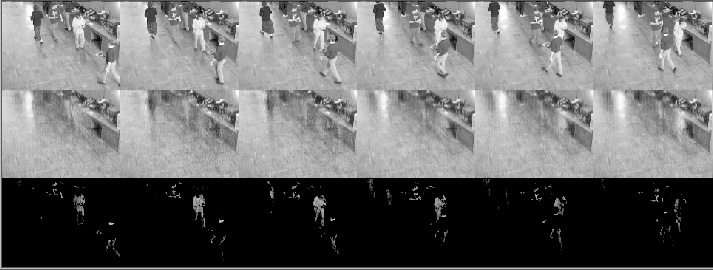
\includegraphics[scale=0.325]{images/Restaurant/CAE_worst.jpg}}
	\subfigure[RPCA.]{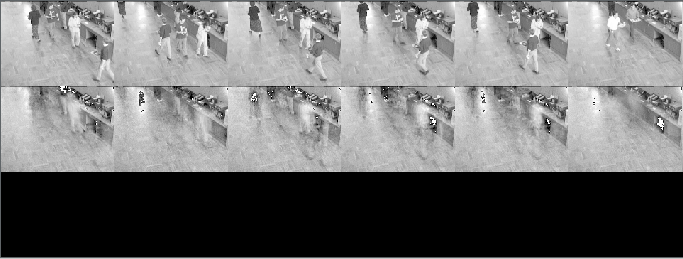
\includegraphics[scale=0.325]{images/Restaurant/RPCA_worst.jpg}}
	\caption{Top anomalous images containing original image (people walking in the lobby) decomposed into background (lobby) and foreground (people), {\tt restaurant} dataset.}
	\label{fig:results-restaurant}
\end{figure}

%\vspace{-0.3 cm}
\textbf{Results}.
While there are no ground truth anomalies in this dataset, a qualitative analysis reveals RCAE to outperforms its counterparts in capturing the foreground objects.
Figure~\ref{fig:results-restaurant} compares the top 6 most anomalous images for RCAE and RPCA.
We see that the most anomalous images contain high foregound activity (which are recognised as anomalous).
Visually, we see that the background reconstruction produced by RPCA contains a few blemishes in some cases, while for RCAE the backgrounds are smooth.


%%%
\subsubsection{{(2) {\tt usps} dataset}}
From the {\tt usps} handwritten digit dataset,
we create a dataset
with a mixture of 220 images of \lq1\rq s, and 11 images of \lq7\rq, as in~\cite{xu2010robust}.
Intuitively, the latter images are treated as being anomalous, as the corresponding images have different characteristics to the majority of the training data. Each image is flattened as a row vector, yielding a 231 $\times$ 256 training matrix.

\textbf{Parameter settings}.
For SVD and RPCA methods, rank $K = 64$ is used.
For AE, the inputs are flattened images as a column vector of size 256,
and the hidden layer is a column vector of size  64 (matching the rank $K$).

For DRMF, we follow the settings of~\cite{xu2010robust}.
For RKPCA, we used a Gaussian kernel with bandwidth $0.01$, a cost parameter $C = 1$, and requested $60\%$ of the KPCA spectrum (which roughly selects 64 principal components).

For RCAE, we set two layers of convolution layers with the filter number to be 32, filter size to be 3$\times$3, with number of strides as $1$ and  rectified linear unit (ReLU) as activation with max-pooling layer of dimension 2$\times$2.

\textbf{Results}.
From Table~\ref{tbl:anomaly-results-summary}, we see that it is a near certainty for all \lq7\rq\, are accurately identified as outliers.
Figure~\ref{fig:usps-anomalies} shows the top anomalous images for RCAE, where indeed the \lq7\rq's are correctly placed at the top of the list.
By contrast, for RPCA there are also some \lq1\rq's placed at the top.

\begin{figure}[!t]
	\centering
	\subfigure[RCAE.]{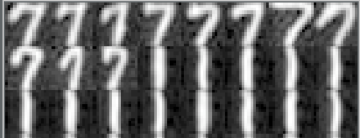
\includegraphics[scale=0.9]{usps-anomalies-crop}}
	\quad
	\subfigure[RPCA.]{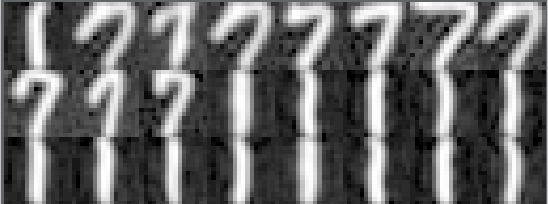
\includegraphics[scale=0.29]{rpca_usps}}
	\caption{Top anomalous images, {\tt usps} dataset.}
	\label{fig:usps-anomalies}
	%\vspace{-\baselineskip}
\end{figure}

\begin{table*}[!t]
	\centering
	\renewcommand{\arraystretch}{1.25}
	\resizebox{0.99\linewidth}{!}{
	\subfigure[{\tt usps}]{
		\begin{tabular}{lccc}
			\toprule
			\toprule
			\textbf{Methods} & \textbf{AUPRC} & \textbf{AUROC} & \textbf{P@10} \\
			\midrule
			RCAE  & \cellcolor{gray!25}{0.9614 $\pm$ 0.0025}&\cellcolor{gray!25}{0.9988$\pm$ 0.0243}&\cellcolor{gray!25}{0.9108 $\pm$ 0.0113} \\
			\midrule
			CAE & 0.7003 $\pm$ 0.0105 & 0.9712 $\pm$ 0.0002 & 0.8730 $\pm$ 0.0023\\
			AE  & 0.8533 $\pm$ 0.0023 & 0.9927 $\pm$ 0.0022 & 0.8108 $\pm$ 0.0003 \\
			\midrule
			RKPCA & 0.5340 $\pm$ 0.0262 & 0.9717 $\pm$ 0.0024 & 0.5250 $\pm$ 0.0307 \\
			DRMF  & 0.7737 $\pm$ 0.0351 & 0.9928 $\pm$ 0.0027 & 0.7150 $\pm$ 0.0342 \\
			RPCA  & 0.7893 $\pm$ 0.0195 & 0.9942 $\pm$ 0.0012 & 0.7250 $\pm$ 0.0323\\
			SVD   & 0.6091 $\pm$ 0.1263 & 0.9800 $\pm$ 0.0105 & 0.5600 $\pm$ 0.0249 \\
			\bottomrule
	\end{tabular}}%
	\quad
	\subfigure[{\tt cifar-10}]{
		\begin{tabular}{ccc}
			\toprule
			\toprule
			\textbf{AUPRC} & \textbf{AUROC} & \textbf{P@10} \\
			\midrule
			\cellcolor{gray!25}{0.9934 $\pm$ 0.0003}&\cellcolor{gray!25}{0.6255 $\pm$ 0.0055} &\cellcolor{gray!25}{0.8716 $\pm$ 0.0005} \\
			\midrule
			0.9011 $\pm$ 0.0000 & 0.6191 $\pm$ 0.0000 & 0.0000 $\pm$ 0.0000 \\
			0.9341 $\pm$ 0.0029 & 0.5260 $\pm$ 0.0003 & 0.2000 $\pm$ 0.0003 \\
			\midrule
			0.0557 $\pm$ 0.0037 & 0.5026 $\pm$ 0.0123 & 0.0550 $\pm$ 0.0185 \\
			0.0034 $\pm$ 0.0000 & 0.4847 $\pm$ 0.0000 & 0.0000 $\pm$ 0.0000 \\
			0.0036 $\pm$ 0.0000 & 0.5211 $\pm$ 0.0000 & 0.0000 $\pm$ 0.0000 \\
			0.0024 $\pm$ 0.0000 & 0.5299 $\pm$ 0.0000 & 0.0000 $\pm$ 0.0000 \\
			\bottomrule
	\end{tabular}}%
	}

	\caption{Comparison between the baseline (bottom four rows) and state-of-the-art systems (top three rows). Results are the mean and standard error of performance metrics over 20 random training set draws. Highlighted cells indicate best performer.}
	\label{tbl:anomaly-results-summary}
	%\vspace{-0.2in}
\end{table*}

\subsubsection{{(3) {\tt cifar-10} dataset}}
We create a dataset with anomalies
by combining 5000 random images of dogs and 50 images of cats, as illustrated in Figure~\ref{fig:results-cifar}.
In this scenario the cats are anomalies, and the goal is to detect all the cats in an unsupervised manner.

\textbf{Parameter settings}.
For SVD and RPCA methods, rank $K = 64$ is used.
We trained a three-hidden-layer autoencoder (AE) (1024-256-64-256-1024 neurons).
The middle hidden layer size is set to be same as rank $K = 64$, %(same as number of components used in SVD and RPCA),
and the model is trained using Adam~\cite{kingma2014adam}.
The decoding layer uses sigmoid function in order to capture the nonlinearity characteristics from  latent representations produced by the hidden layer.
Finally, we obtain the feature vector for each image by obtaining the latent representation from the hidden layer.

For RKPCA, we used a Gaussian kernel with bandwidth $5 \cdot 10^{-8}$, a cost parameter $C = 0.1$, and requested $55\%$ of the KPCA spectrum (which roughly selects 64 principal components).
The RKPCA runtime was prohibitive on the full sample (see Sec \ref{sec:runtime}), so we resorted to a subsample of 1000 dogs and 50 cats.

The RCAE architecture in this experiment is same as for {\tt restaurant}, containing
four layers of  (conv-batch-normalization-elu) in the encoder part
and four layers of  (conv-batch-normalization-elu) in the decoder
portion of the network. RCAE network parameters such as (number of filter, filter size, strides) are chosen to be (16,3,1)  for first and second layers and (32,3,1) for third and fourth layers of both encoder and decoder.

\begin{figure}[!t]
	\centering
	\subfigure[RCAE.]{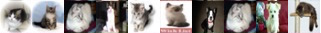
\includegraphics[scale=0.95]{images/CIFAR_10/CAE_worst_inductive_crop}}
	\subfigure[RPCA.]{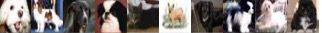
\includegraphics[scale=0.95]{images/CIFAR_10/RPCA_worst_inductive_crop}}
	\caption{Top anomalous images, %along with background and foreground,
	{\tt cifar-10} dataset.}
	\label{fig:results-cifar}
\end{figure}

\textbf{Results}.
From Table \ref{tbl:anomaly-results-summary},
RCAE clearly outperforms all existing state-of-the art methods in anomaly detection.
Note that basic CAE, with no robustness (effectively $\lambda = \infty$), is also outperformed by our method, indicating that it is crucial to explicitly handle anomalies with the $\N$ term.

Figure~\ref{fig:results-cifar} illustrates the most anomalous images for our RCAE method, compared to RPCA.
Owing to the latter involving learning a linear subspace, the model is unable to effectively distinguish cats from dogs;
by contrast, RCAE can effectively determine the manifold characterising most dogs, and identifies cats to be anomalous with respect to this.


%%%%%%%%%
\subsection{Inductive anomaly detection results}

We conduct an experiment to assess the detection of \emph{inductive} anomalies.
Recall that this is a capability of our RCAE model, but not e.g. RPCA.
We consider the following setup:
we train our model on 5000 dog images, and then evaluate it on a test set comprising 500 dogs and 50 cat images.
As before, we wish all methods to accurately determine the cats to be anomalies.

\begin{figure}[!t]
	\centering
	\subfigure[RCAE.]{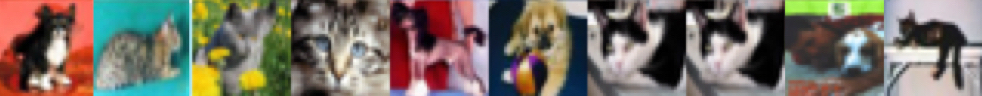
\includegraphics[scale=0.31]{images/CIFAR_10/caeInductiveAnomalies_crop.jpg}}
	\subfigure[CAE.]{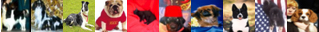
\includegraphics[scale=0.95]{images/CIFAR_10/caeInductiveAnomalies_crop_new.jpg}}
	\caption{Top inductive anomalous images, {\tt cifar-10} dataset.}
	\label{fig:results-cifar-inductive}
\end{figure}


Table~\ref{tbl:inductive-anomaly-results} summarises the detection performance for all the methods on this inductive task.
The lower values compared to Table~\ref{tbl:anomaly-results-summary} are indicative that the problem here is more challenging than anomaly detection on a single dataset;
nonetheless, we see that our RCAE method manages to convincingly outperform both the SVD and AE baselines.
This is confirmed qualitatively in Figure~\ref{fig:results-cifar-inductive}, where we see that RCAE correctly identifies many cats in the test set as anomalous, while the basic
%AE
CAE
method suffers.

\begin{table}[!t]
	\centering
	\renewcommand{\arraystretch}{1.25}
	\caption{Inductive anomaly detection results on {\tt cifar-10}. Note that RPCA and DRMF are inapplicable here. Highlighted cells indicate best performer.}
	\resizebox{0.99\linewidth}{!}{
	\begin{tabular}{@{}lccccc@{}}
		\toprule
		\toprule
		& \textbf{SVD} & \textbf{RKPCA} & \textbf{AE} & \textbf{CAE} & \textbf{RCAE} \\
		\toprule
		\bf{AUPRC} & 0.1752 $\pm$ 0.0051 & 0.1006 $\pm$ 0.0045 & 0.6200 $\pm$ 0.0005 & 0.6423 $\pm$ 0.0005 & \cellcolor{gray!25}{0.6908 $\pm$ 0.0001} \\
		\bf{AUROC} & 0.4997 $\pm$ 0.0066 & 0.4988 $\pm$ 0.0125 & 0.5007 $\pm$ 0.0010 & 0.4708 $\pm$ 0.0003 & \cellcolor{gray!25}{0.5576 $\pm$ 0.0005} \\
		\bf{P@10}  & 0.2150 $\pm$ 0.0310 & 0.0900 $\pm$ 0.0228 & 0.1086 $\pm$ 0.0001 & 0.2908 $\pm$ 0.0001 & \cellcolor{gray!25}{0.5986 $\pm$ 0.0001} \\
		\bottomrule
	\end{tabular}
	}
	\label{tbl:inductive-anomaly-results}
\end{table}


%%%
\subsection{Image denoising results}

Finally, we test the ability of the model to de-noise images, which is a form of anomaly detection on individual pixels (or more generally, features).
In this experiment, we train all models on a set of 5000 images of dogs from {\tt cifar-10}.
For each image, we then add salt-and-pepper noise at a rate of 10\%.
Our goal is to recover the original image as accurately as possible.

Figure~\ref{fig:results-cifar-injection} illustrates that the most anomalous images in the presence of noise
contain images of the variations of dog class images (e.g. containing person's face).
Further, Figure \ref{fig:denoising-results} illustrates for various methods the mean square error between the reconstructed and original images.
RCAE effectively suppresses the noise as evident from the low error.
The improvement over raw CAE is modest, but suggests that there is benefit to explicitly accounting for noise.

%\vspace{-0.3 cm}
\begin{figure}[!t]
	\centering
	\subfigure[RCAE.]{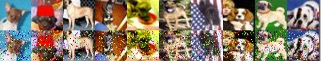
\includegraphics[scale=0.95]{images/CIFAR_10/CAE_worst_crop.jpg}}
	\subfigure[RPCA.]{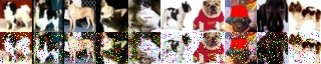
\includegraphics[scale=0.95]{images/CIFAR_10/RPCA_worst_crop.jpg}}
	\caption{Top anomalous images in original form (first row), noisy form (second row),
	image denoising task on {\tt cifar-10}.}
	\label{fig:results-cifar-injection}
\end{figure}

\begin{figure}[!t]
	\centering
	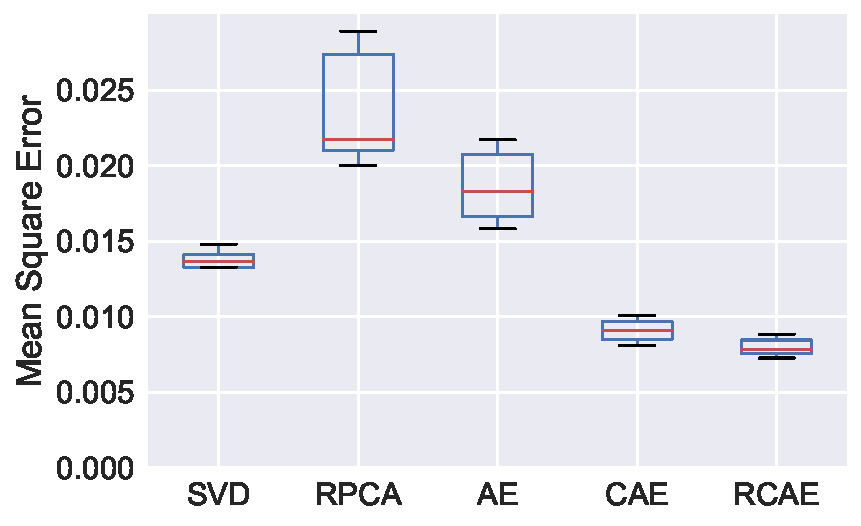
\includegraphics[scale=0.5]{images/cifar_10_mse.pdf}
	\caption{Illustration of the mean square error boxplots obtained for various models on image denoising task, {\tt cifar-10} dataset.
		In this setting, RCAE suppresses the noise and detects the background and foreground images effectively.}
	\label{fig:denoising-results}
	%\vspace{-\baselineskip}
\end{figure}


%%%
\subsection{Comparison of training times}
\label{sec:runtime}

We remark finally that our RCAE method is comparable in training efficiency to existing methods.
For example, on the small-scale {\tt restaurant} dataset, it takes 1 minute to train RPCA,
and 8.5 minutes to train RKPCA,
compared with 10 minutes for our RCAE method.
The ability to leverage recent advances in deep learning as part of our optimisation (e.g.\ training models on a GPU) is we believe a salient feature of our approach.

We note that while the RKPCA method is fast to train on smaller datasets, on larger datasets it suffers from the $O(n^2)$ complexity of kernel methods;
for example, it takes over an hour to train on the {\tt cifar-10} dataset.
It is plausible that one could leverage recent advances in fast approximations of kernel methods~\cite{Lopez-Paz:2014}, and studying these would be of interest in future work.
Note that the issue of using a fixed kernel function would remain, however.
